\newpage
\section*{Avancement} % (2 pages) Diagramme de gant avec planning prévisionnel

Voici le diagramme de Gantt prévisionnel : 

\begin{figure}[H]
  \centering
  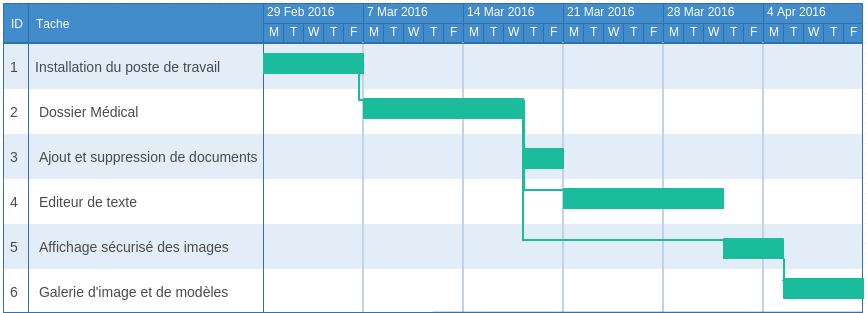
\includegraphics[width=17cm]{./img/gantt_prev}
  \caption{\label{fig:mb_va_ast} Gantt prévisionnel.}
\end{figure}

Et voici le diagramme de gantt réel : 

\begin{figure}[H]
  \centering
  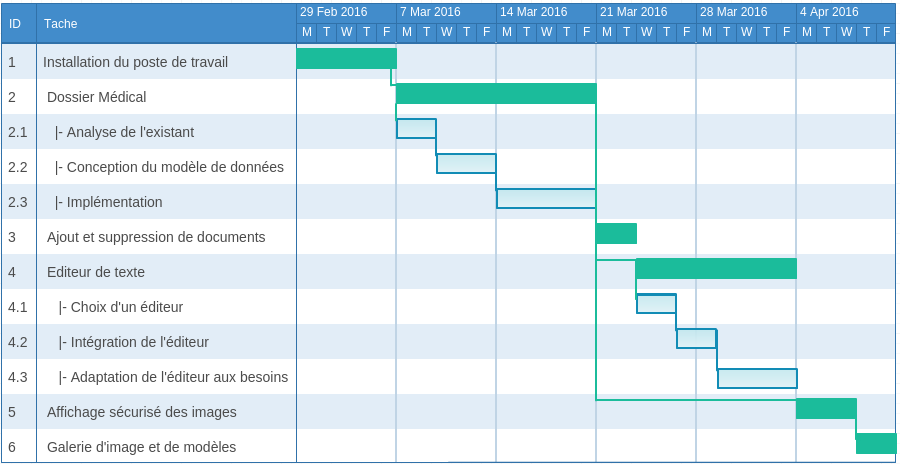
\includegraphics[width=17cm]{./img/gantt_reel}
  \caption{\label{fig:mb_va_ast} Gantt réel.}
\end{figure}

%TODO Planning prévisionnel 
%TODO Planning réalisé + explications

% TODO définition des tâches 
%TODO Différences prévisionnel/réalisé
%TODO Tâches particulières

%TODO Outils d'assistance au développement utilisés.

%TODO Méthode de travail employée : méthode de développement, mode de travail en équipe, réunions-présentations etc.

%TODO Si travail en mode agile, inclure une analyse de la méthode de travail, (identifier ce qui était prévu au départ au niveau macro, l'implémentation effective, les virages pris après chaque sprint après les retours clients).

%TODO Faites une évaluation du coût du projet que vous avez réalisé (en environné), si besoin faites vous aider par votre tuteur en entreprise. 